\documentclass{beamer}
\mode<presentation>
\usetheme{Madrid}
\usepackage{amsfonts,amsmath,amsthm,amssymb}
\usepackage{graphicx,graphics,listings}
\usepackage{setspace,fontspec,caption}
\usepackage[utf8x]{inputenc}
\newcommand*{\utb}{\item[{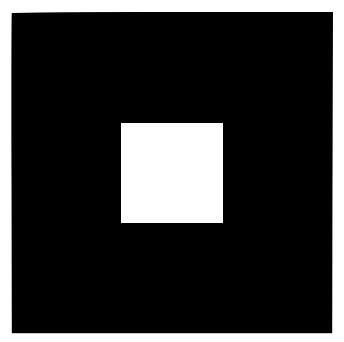
\includegraphics[width=0.3cm]{img/UTSymbols-Bullet.png}}]}
\renewcommand*{\thefootnote}{\fnsymbol{footnote}}
\newcommand{\sign}[1]{\ensuremath{\operatorname{sign(\mathit{#1})}}}

\newfontfamily{\lstIBMPlexMono}[Path = fonts/, UprightFont=IBMPlexMono-Medium.otf, BoldFont=IBMPlexMono-Bold.otf]{}
\setsansfont[Path = fonts/, UprightFont=UTSans-Medium.otf, BoldFont=UTSans-Bold.otf]{}
\lstset{basicstyle=\lstIBMPlexMono\scriptsize,language=C++}

\title{\bf The Nearest Neighbor Algorithm}
\author[hello@msirbu.eu]{Sîrbu Matei-Dan}
\institute[]{Transilvania University of Brașov \\ The Faculty of Mathematics and Computer Science}
\date{17 December 2020}

\definecolor{albastruMI}{rgb}{0, 0.23, 0.49}
\setbeamercolor*{palette primary}{bg=albastruMI, fg = white}
\setbeamercolor*{palette secondary}{bg=albastruMI, fg = white}
\setbeamercolor*{palette ternary}{bg=albastruMI, fg = white}
\setbeamercolor*{palette quaternary}{bg=albastruMI, fg = white}
\setbeamercolor*{author in head/foot}{parent=palette primary}
\usefonttheme[onlymath]{serif}

\begin{document}
\frame{\titlepage}

\begin{frame}
    \frametitle{The Nearest Neighbor Algorithm}
    \setstretch{1.5}
    \begin{itemize}
        \utb Hypothesis Space
        \begin{itemize}
            \utb variable size
            \utb deterministic
            \utb continuous parameters
        \end{itemize}
    \end{itemize}
    \begin{itemize}
        \utb Learning Algorithm
        \begin{itemize}
            \utb direct computation
            \utb lazy
        \end{itemize}
    \end{itemize}
\end{frame}

\begin{frame}
    \frametitle{Nearest Neighbor Algorithm}
    \begin{itemize}
        \utb Store all of the training examples
        \utb Classify a new example $\mathbf{x}$ by finding the training example $\langle \mathbf{x}_i, y_i \rangle$ that is nearest to $\mathbf{x}$ according to Euclidean distance: $$\lVert \mathbf{x} - \mathbf{x}_i \rVert = \sqrt{\sum_j (x_j - x_{ij})^2}$$
        guess the class $\hat{y} = y_i$.
        \utb Efficiency trick: squared Euclidean distance gives the same answer but avoids the square root computation $$\lVert \mathbf{x} - \mathbf{x}_i \rVert^2 = \sum_j (x_j - x_{ij})^2$$
    \end{itemize}
\end{frame}

\begin{frame}
    \frametitle{Decision Boundaries: The Voronoi Diagram}
    \begin{center}
        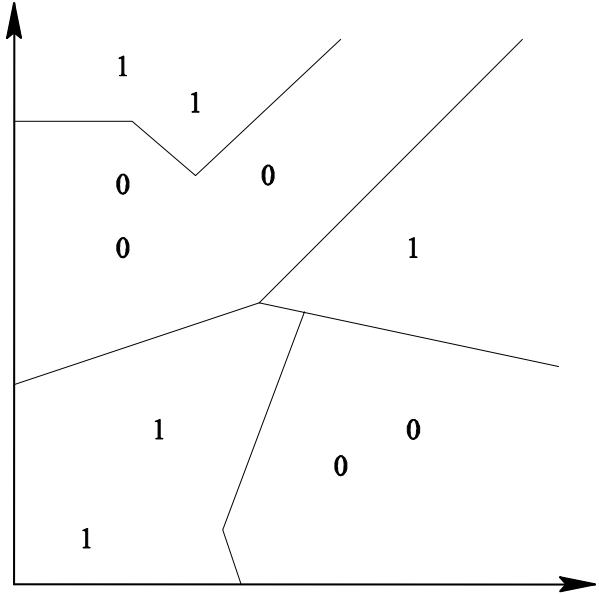
\includegraphics[width=0.3\textwidth]{img/1}
    \end{center}
    \begin{itemize}
        \utb Nearest Neighbor does not explicitly compute decision boundaries. However, the boundaries form a subset of the Voronoi diagram of the training data
        \utb Each line segment is equidistant between two point of opposite class. The more examples that are stored, the more complex the decision boundaries can become.
    \end{itemize}
\end{frame}

\begin{frame}
    \frametitle{Nearest Neighbor depends critically on the distance metric}
    \begin{itemize}
        \utb Normalize Feature Values:
        \begin{itemize}
            \utb All features should have the same range of values (e.g. $[-1, +1]$). Otherwise, features with larger ranges will be treated as more important
        \end{itemize}
        \utb Remove Irrelevant Features:
        \begin{itemize}
            \utb Irrelevant or noisy features add random perturbations to the distance measure and hurt performance
        \end{itemize}
        \utb Learn a Distance Metric:
        \begin{itemize}
            \utb One approach: weight each feature by its mutual information with the class. Let $w_j = l(x_j;y)$. Then $d(\mathbf{x},\mathbf{x'}) = \sum_{j=1}^n w_j(x_j - x'_j)^2$
            \utb Another approach: use the Mahalanobis distance: $D_M(\mathbf{x},\mathbf{x'}) = (\mathbf{x} - \mathbf{x'})^\top \sum^{-1} (\mathbf{x} - \mathbf{x'})$
        \end{itemize}
        \utb Smoothing:
        \begin{itemize}
            \utb Find the $k$ nearest neighbors and have them vote. This is especially good when there is noise in the class labels.
        \end{itemize}
    \end{itemize}
\end{frame}

\begin{frame}
    \frametitle{$k$-d tree}
    \begin{itemize}
        \utb A $k$-d tree is similar to a decision tree except that we split using the \textit{median} value along the dimension having the \textit{highest variance}. Every internal node stores one data point, and the leaves are empty
    \end{itemize}
    \begin{center}
        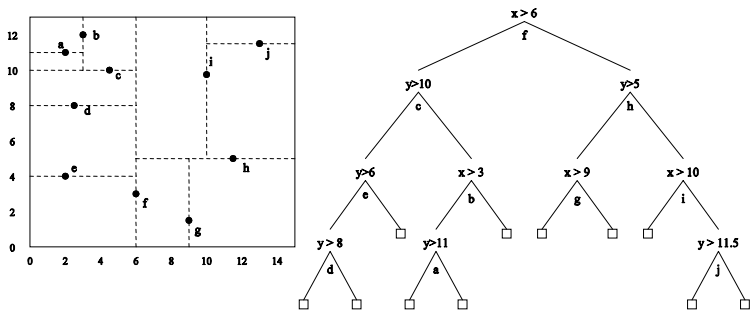
\includegraphics[width=0.9\textwidth]{img/2}
    \end{center}
\end{frame}

\begin{frame}[fragile]
    \frametitle{$\log$ time queries with $k$-d trees}
    \begin{lstlisting}
        KDTree root;
        Node NearestNeighbor(Point P)
        {
            PriorityQueue PQ; // minimizing queue
            float bestDist = infinity; // smallest distance seen so far
            Node bestNode; // nearest neighbor so far
            PQ.push(root, 0);
            while (!PQ.empty()) {
                (node, bound) = PQ.pop();
                if (bound >= bestDist) return bestNode.p;
                float dist = distance(P, node.p);
                if (dist < bestDist) {bestDist = dist; bestNode = node;}
                if (node.test(P)) {
                    PQ.push(node.left, P[node.feat] - node.thresh);
                    PQ.push(node.right, 0);
                }
                else {
                    PQ.push(node.left, 0);
                    PQ.push(node.right, node.thresh - P[node.feat]);
                }
            } // while
            return bestNode.p;
        } // NearestNeighbor
    \end{lstlisting}
\end{frame}

\begin{frame}
    \frametitle{Example}
    \begin{center}
        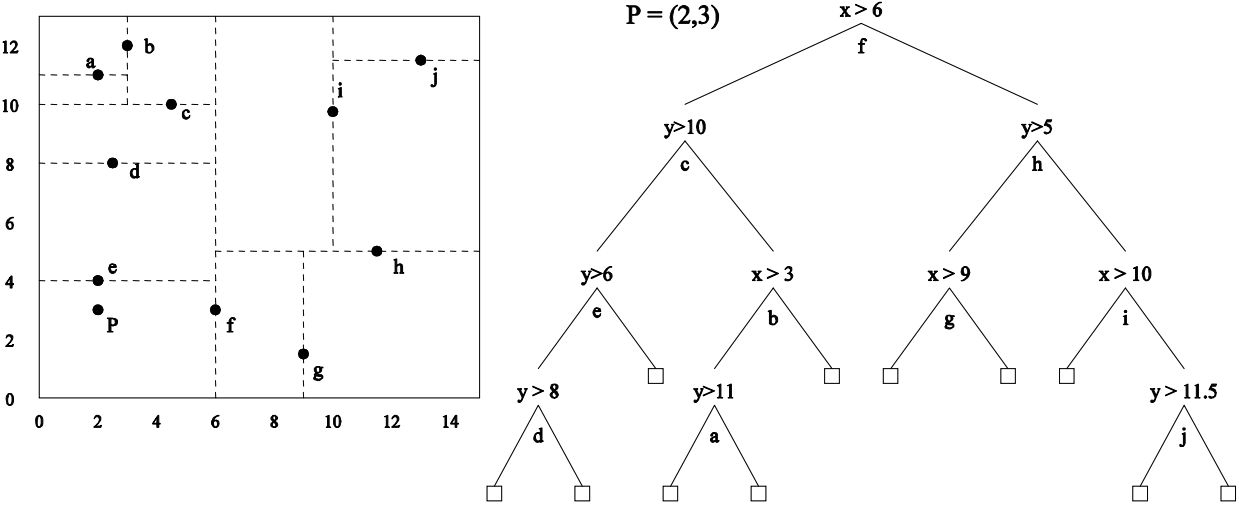
\includegraphics[width=0.7\textwidth]{img/3}
        \begin{tabular}{|c|c|c|l|}
            \hline
            New Distance & Best Distance & Best node & Priority Queue \\
            \hline
            none & $\infty$ & none & $(f,0)$ \\ \hline
            4.00 & 4.00 & $f$ & $(c,0) (h,4)$ \\ \hline
            7.61 & 4.00 & $f$ & $(e,0) (h,4) (b,7)$ \\ \hline
            1.00 & 1.00 & $e$ & $(d,1) (h,4) (b,7)$ \\ \hline
        \end{tabular}
    \end{center}
    \begin{itemize}
        \utb This is a form of A* search using the minimum distance to a node as an underestimate of the true distance
    \end{itemize}
\end{frame}

\begin{frame}
    \frametitle{Filter Pipeline}
    \setstretch{1.5}
    \begin{itemize}
        \utb Consider several distance measures: $D_1, D_2, \dots, D_n$ where $D_{i+1}$ is more expensive to compute than $D_i$
        \utb Calibrate a threshold $N_i$ for each filter using the training data
        \utb Apply the nearest neighbor rule with $D_i$ to compute the $N_i$ nearest neighbors
        \utb Then apply filter $D_{i+1}$ to those neighbors and keep the $N_{i+1}$ nearest, and so on
    \end{itemize}
\end{frame}

\begin{frame}
    \frametitle{The Curse of Dimensionality}
    \begin{itemize}
        \utb Nearest neighbor breaks down in high-dimensional spaces, because the "neighborhood" becomes very large.
        \utb Suppose we have $5000$ points uniformly distributed in the unit hypercube and we want to apply the 5-nearest neighbor algorithm. Suppose our query point is at the origin.
        \utb Then on the 1-dimensional line, we must go a distance of $5/5000 = 0.001$ on the average to capture the 5 nearest neighbors
        \utb In 2 dimensions, we must go $\sqrt{0.001}$ to get a square that contains $0.001$ of the volume.
        \utb In $D$ dimensions, we must go $(0.001)^{1/d}$
    \end{itemize}
    \begin{center}
        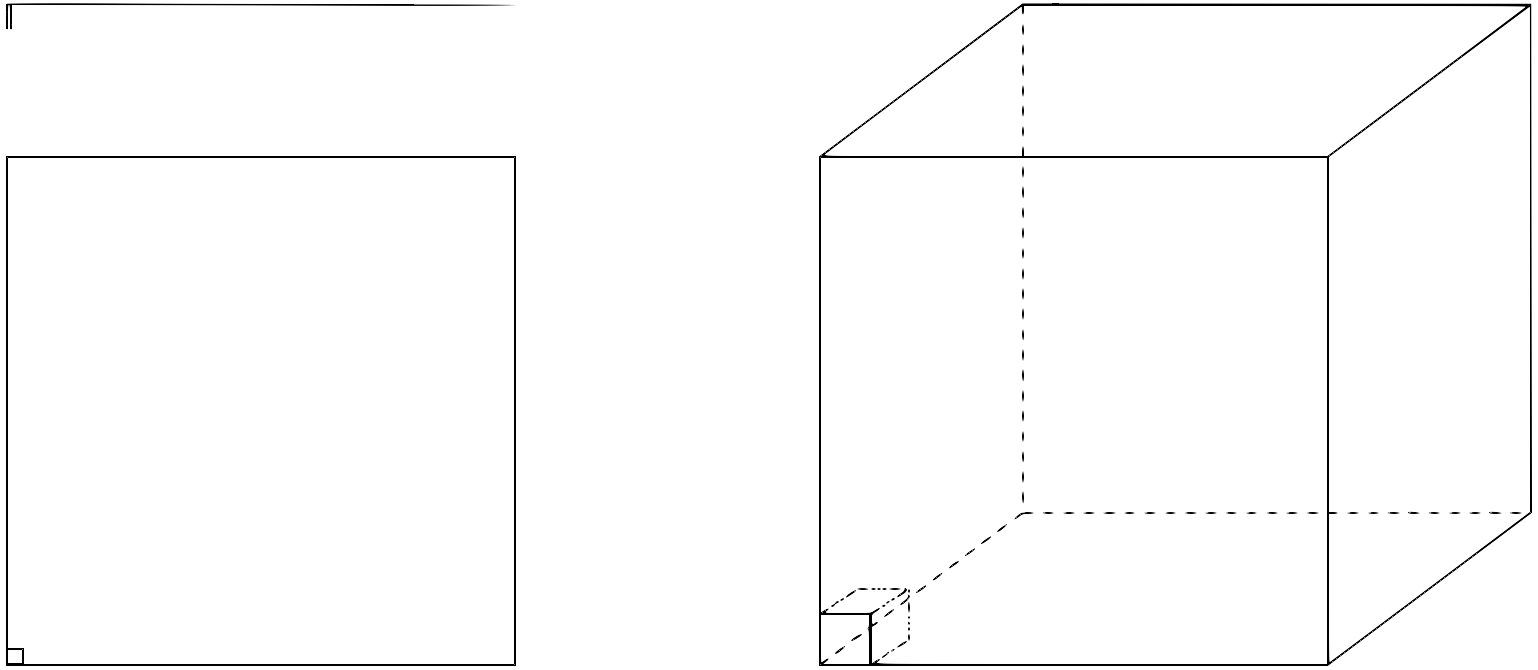
\includegraphics[width=0.5\textwidth]{img/4}
    \end{center}
\end{frame}

\begin{frame}
    \frametitle{The Curse of Dimensionality (2)}
    \begin{itemize}
        \utb With $5000$ points in $10$ dimensions, we must go $0.501$ distance along each attribute in order to find the 5 nearest neighbors
    \end{itemize}
    \begin{center}
        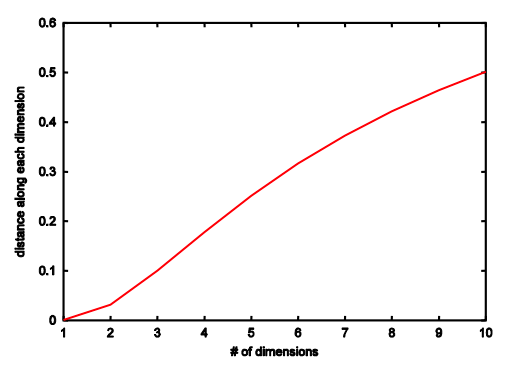
\includegraphics[width=0.7\textwidth]{img/5}
    \end{center}
\end{frame}

\begin{frame}
    \frametitle{The Curse of Noisy/Irrelevant Features}
    \begin{itemize}
        \utb NNbr also breaks down when the data contains irrelevant, noisy features.
        \utb Consider a 1D problem where our query $x$ is at the origin, our nearest neighbor is $x_1$ at $0.1$, and our second nearest neighbor is $x_2$ at $0.5$.
        \utb Now add a uniformly random noisy feature. What is the probability that $x_2'$ will now be closer to $x$ and $x_1'$? Approximately $0.15$.
    \end{itemize}
    \begin{center}
        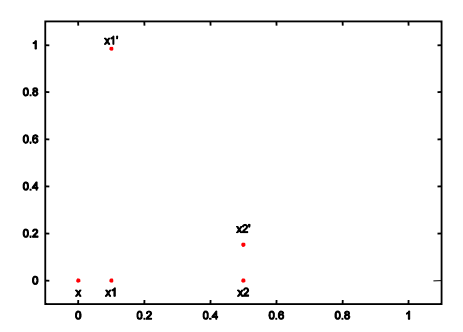
\includegraphics[width=0.5\textwidth]{img/6}
    \end{center}
\end{frame}

\begin{frame}
    \frametitle{The Curse of Noise (2)}
    \begin{center}
        \Large Location of $x_1$ versus $x_2$ \\
        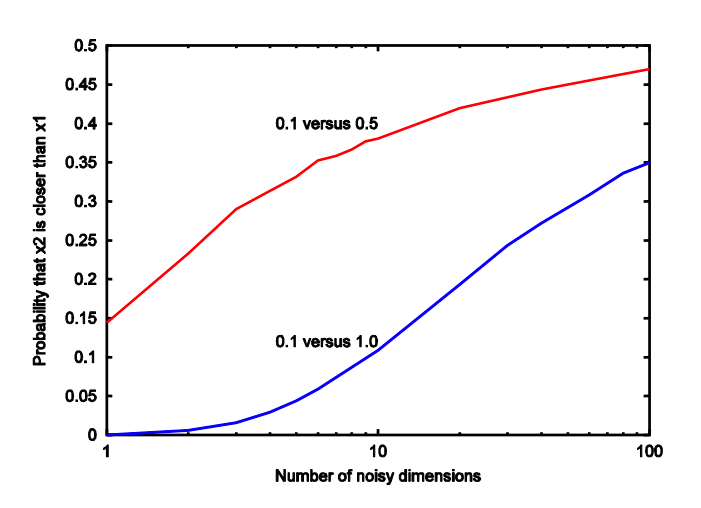
\includegraphics[width=0.75\textwidth]{img/7}
    \end{center}
\end{frame}

\begin{frame}
    \frametitle{Nearest Neighbor Evaluation}
    \resizebox{1\textwidth}{!}{
    \begin{tabular}{lllllll}
        Criterion & Perc & Logistic & LDA & Trees & Nets & NNbr \\
        \hline 
        Mixed data & no & no & no & yes & no & no \\
        Missing values & no & no & yes & yes & no & somewhat \\
        Outliers & no & yes & no & yes & yes & yes \\
        Monotone transformations & no & no & no & yes & somewhat & no \\
        Scalability & yes & yes & yes & yes & yes & no \\
        Irrelevant inputs & no & no & no & somewhat & no & no \\
        Linear combinations & yes & yes & yes & no & yes & somewhat \\
        Interpretable & yes & yes & yes & yes & no & no \\
        Accurate & yes & yes & yes & no & yes & no
    \end{tabular}
    }
\end{frame}

\begin{frame}
    \frametitle{Nearest Neighbor Summary}
    \setstretch{1.5}
    \begin{itemize}
        \utb Advantages
        \begin{itemize}
            \utb variable-sized hypothesis space
            \utb learning is extremely efficient and can be online or batch
            \begin{itemize}
                \utb However, growing a good $k$-d tree can be expensive
            \end{itemize}
            \utb Very flexible boundaries
        \end{itemize}
        \utb Disadvantages
        \begin{itemize}
            \utb distance function must be carefully chosen
            \utb irrelevant or correlated features must be eliminated
            \utb typically cannot handle more than 30 features
            \utb computational costs: memory and classification-time computation
        \end{itemize}
    \end{itemize}
\end{frame}

\end{document}